\chapter{Specifikacija programske potpore}
		
	\section{Funkcionalni zahtjevi}
			\noindent \textbf{Dionici:}
			
			\begin{packed_enum}
				
				\item Vlasnik (naručitelj)
				\item Neregistrirani korisnik
				\item Roditelji				
				\item Liječnici i pedijatri
				\item Administrator
				\item Razvojni tim
				
			\end{packed_enum}
			
			\noindent \textbf{Aktori i njihovi funkcionalni zahtjevi:}
			
			
			\begin{packed_enum}
				\item  \underbar{Neregistrirani/neprijavljeni korisnik (inicijator) može:}
				
				\begin{packed_enum}
					
					\item pregledati katalog usluga aplikacije
					\item vidjeti koje sve vrste korisnika aplikacija podržava
					\item registrirati se u sustav, koristeći korisničko ime, email adresu, lozinku, ime, prezime i OIB, čime stvara osobni korisnički račun
					\item prijaviti se u sustav putem korisničkog imena i lozinke
					
				\end{packed_enum}
			
				\item  \underbar{Roditelj (inicijator) može:}
				
				\begin{packed_enum}
					
					\item pristupiti profilima svoje djece ili svojem profilu
					\item otvarati i čitati obavijesti vezane uz svaki profil, poslane od liječnika ili pedijatra
					\item vidjeti svoj ili djetetov medicinski karton te povijest pregleda
					\item pristupiti ispričnicama generiranim za pojedino dijete te potvrdama o bolovanju
					\item pristupiti naknadnim nalazima laboratorijskih pretraga
					\item primiti informacije i narudžbe na specijalističke preglede, te vidjeti lokacije na kojima je moguće izvesti navedeni pregled
					\item učitati (\textit{uploadati}) nalaze koje dobije prilikom pregleda u privatnoj ordinaciji
					
				\end{packed_enum}
				
				\item  \underbar{Pedijatar (inicijator) može:}
				
				\begin{packed_enum}
					
					\item pristupiti profilima djece kojima je dedicirani pedijatar
					\item pristupiti liječničkim kartonima svih svojih pacijenata
					\item prijaviti novo dijete prilikom prvog pregleda, koristeći osobne podatke djeteta (ime, prezime, OIB, datum rođenja), te OIB roditelja
					\item za svakog pacijenta unijeti novi pregled
					\item za svakog pacijenta generirati ispričnicu
					\item za roditelje djece preporučiti bolovanje
					\item naručiti dijete na specijalistički pregled, te preporučiti lokacije za izvedbu istog
					
				\end{packed_enum}
				
				\item  \underbar{Liječnik obiteljske medicine(inicijator) može:}
				
				\begin{packed_enum}
					
					\item pristupiti profilima roditelja kojima je liječnik
					\item pristupiti liječničkim kartonima svih svojih pacijenata
					\item za svakog pacijenta unijeti novi pregled
					\item potvrditi ili odbiti preporuke za bolovanje roditelja
					\item naručiti roditelja na specijalistički pregled, te preporučiti lokacije za izvedbu istog
					
				\end{packed_enum}
				
				\item  \underbar{Administrator(inicijator) može:}
				
				\begin{packed_enum}
					
					\item vidjeti popis svih registriranih korisnika i njihovih osobnih podataka
					\item brisati korisnike
					\item mijenjati veze između korisnika, npr. premjestiti dijete s profila jednog roditelja na profil drugog
					\item stvarati profile liječnika i pedijatara
					
				\end{packed_enum}
				
				\item  \underbar{Baza podataka(sudionik):}
				
				\begin{packed_enum}
					
					\item pohranjuje sve podatke o korisnicima, njihove međusobne povezanosti i uloge
					\item pohranjuje liječničke kartone i dijagnoze roditelja i djece
					
				\end{packed_enum}
				
			\end{packed_enum}
			
			\eject 
			
			
				
			\subsection{Obrasci uporabe}
					\noindent \underbar{\textbf{UC1 - Pregledaj usluge aplikacije}}
					\begin{packed_item}
	
						\item \textbf{Glavni sudionik: }Neprijavljeni korisnik
						\item  \textbf{Cilj:} Upoznati se s mogućnostima aplikacije
						\item  \textbf{Sudionici:}-
						\item  \textbf{Preduvjet:}-
						\item  \textbf{Opis osnovnog tijeka:}
						
						\item[] \begin{packed_enum}
	
							\item Korisnik otvara web stranicu aplikacije
							\item Korisnik pregledava sadržaj stranice
						\end{packed_enum}
						\item  \textbf{Opis mogućih odstupanja:}
						\item[] \begin{packed_item}
						
							\item[1.a] Neuspjeh učitavanja stranice, zbog greške u pristupu serverima
							\item[] \begin{packed_enum}
							
								\item Korisnika se obavještava o neuspjehu učitavanja stranice putem ispisane poruke
								\item Korisnik provjerava svoj pristup internetu, te pokušava ponovno
							
							\end{packed_enum}
						\end{packed_item}
					\end{packed_item}
					\noindent \underbar{\textbf{UC2-Registriraj se}}
					\begin{packed_item}
						
						\item \textbf{Glavni sudionik: }Neregistrirani korisnik
						\item  \textbf{Cilj:} Stvoriti korisnički račun roditelja za prijavu u sustav
						\item  \textbf{Sudionici:} Baza podataka
						\item  \textbf{Preduvjet:} Otvorena početna stranica aplikacije
						\item  \textbf{Opis osnovnog tijeka:}
						
						\item[] \begin{packed_enum}
							
							\item Na početnoj stranici aplikacije korisnik odabire opciju "Registriraj se"
							\item Sustav otvara ekran registracije
							\item Korisnik unosi osobne i korisničke podatke, te potvrđuje da se želi registrirati
							\item Sustav ažurira bazu podataka i vraća korisnika na početnu stranicu
							\item Korisnik prima vizualnu obavijest o registraciji
						\end{packed_enum}
						
						\item  \textbf{Opis mogućih odstupanja:}
						\item[] \begin{packed_item}
							\item[3.a] Odabir već korištenog korisničkog imena, email-a ili OIB-a/nepravilan format unosa
							\item[] \begin{packed_enum}
								\item Korisnika se obavještava o neuspjehu registracije, i vraća ga se na stranicu za registraciju
								\item Korisnik ispravlja nepravilno unesene podatke, te ponovno potvrđuje unos
							\end{packed_enum}
							\item[3.b] Korisnik odabire opciju "Odustani"
							\item[] \begin{packed_enum}
								\item Sustav korisnika vraća na početnu stranicu (korak 1)
							\end{packed_enum}
							
						\end{packed_item}
					\end{packed_item}
					
					\noindent \underbar{\textbf{UC3 - Prijavi se u sustav}}
					\begin{packed_item}
						
						\item \textbf{Glavni sudionik: }Roditelj/Pedijatar/Liječnik obiteljske medicine
						\item  \textbf{Cilj:} Prijava u sustav čime se pristupa korisničkom profilu
						\item  \textbf{Sudionici:} Baza podataka
						\item  \textbf{Preduvjet:} Registracija roditelja, postojanje profila pedijatra i liječnika u sustavu
						\item  \textbf{Opis osnovnog tijeka:}
						
						\item[] \begin{packed_enum}
							
							\item Korisnik odabire opciju "Prijava" na početnoj stranici aplikacije
							\item Sustav otvara ekran prijave
							\item Korisnik unosi svoje korisničko ime i lozinku, te odabire opciju "Prijavi se"
							\item Nakon provjere unesenih podataka u bazi podataka, sustav korisniku otvara početna stranica profila
						\end{packed_enum}
						
						\item  \textbf{Opis mogućih odstupanja:}
						
						\item[] \begin{packed_item}
							\item[3.a] Korisnik odabire opciju "Odustani"
							\item[] \begin{packed_enum}
								\item Sustav korisnika vraća na početnu stranicu (korak 1)
							\end{packed_enum}
							\item[4.a] Nepravilan unos imena ili lozinke
							\item[] \begin{packed_enum}
								
								\item Korisnik dobiva informaciju o neuspjeloj prijavi, i vraća ga se na stranicu za prijavu
								\item Korisnik ispravlja nepravilno unesene podatke
								
							\end{packed_enum}
						\end{packed_item}
					\end{packed_item}
					
					\noindent \underbar{\textbf{UC4 - Pregledaj obavijesti (1)}}
					\begin{packed_item}
						
						\item \textbf{Glavni sudionik: }Roditelj
						\item  \textbf{Cilj:} Informiranje roditelja o svim novostima vezanim uz profile njih i djece
						\item  \textbf{Sudionici:} Baza podataka
						\item  \textbf{Preduvjet:} Prijava roditelja u sustav
						\item  \textbf{Opis osnovnog tijeka:}
						
						\item[] \begin{packed_enum}
							
							\item Sustav uzima popis obavijesti iz baze podataka i prikazuje korisniku
							\item Roditelj čita popis obavijesti (vezanih uz sve profile računa roditelja, dakle osobni profil i sva djeca) koji mu se prikazuje na lijevoj strani sučelja nakon uspješne prijave
							
						\end{packed_enum}
						\item  \textbf{Opis mogućih odstupanja:}
						
						\item[] \begin{packed_item}
							
							\item[1.a] Greška pri pristupu obavijestima u bazi podataka
							\item[] \begin{packed_enum}
								
								\item Roditelja se obavještava o neuspjehu dohvaćanja obavijesti, putem ispisane poruke
								\item Roditelja se moli da pokuša kasnije, ili da kontaktira administratora
								
							\end{packed_enum}
						\end{packed_item}
					\end{packed_item}
					
					\noindent \underbar{\textbf{UC5 - Odaberi profil}}
					\begin{packed_item}
						
						\item \textbf{Glavni sudionik: }Roditelj
						\item  \textbf{Cilj:} Pristup podacima i funkcijama pojedinog profila roditelja ili djeteta
						\item  \textbf{Sudionici:} Baza podataka
						\item  \textbf{Preduvjet:} Prijava roditelja u sustav
						\item  \textbf{Opis osnovnog tijeka:}
						
						\item[] \begin{packed_enum}
							
							\item Sustav filtrira popis profila vezanih uz roditeljski račun iz baze podataka, te ih prikazuje
							\item Roditelj odabire jedan od profila koji mu se prikazuju na desnoj strani sučelja nakon uspješne prijave
							\item Sustav pronalazi podatke o kliknutom profilu, te otvara stranicu odabranog profila
							
						\end{packed_enum}
						\item  \textbf{Opis mogućih odstupanja:}
						\item[] \begin{packed_item}
							
							\item[1.a] Greška u sustavu pri pristupu odabranom profilu
							\item[] \begin{packed_enum}
								
								\item Roditelja se obavještava o neuspjehu dohvaćanja podataka o profilu, putem ispisane poruke
								\item Roditelja se moli da pokuša kasnije, ili da kontaktira administratora
								
							\end{packed_enum}
						\end{packed_item}
						
					\end{packed_item}
					
					\noindent \underbar{\textbf{UC6 - Pregledaj obavijesti (2)}}
					\begin{packed_item}
						
						\item \textbf{Glavni sudionik: }Roditelj
						\item  \textbf{Cilj:} Informiranje roditelja o novostima vezanim uz odabrani profil
						\item  \textbf{Sudionici:} Baza podataka
						\item  \textbf{Preduvjet:} Odabir profila djeteta ili roditelja
						\item  \textbf{Opis osnovnog tijeka:}
						
						\item[] \begin{packed_enum}
							\item Sustav uzima popis obavijesti iz baze podataka te ih prikazuje
							\item Roditelj čita popis obavijesti (isključivo vezanih za odabrani profil) koji mu se prikazuje na desnoj strani sučelja nakon uspješne odabira profila \\

						\end{packed_enum}
						\item  \textbf{Opis mogućih odstupanja:}
						\item[] \begin{packed_item}
							
							\item[1.a] Greška pri pristupu obavijestima u bazi podataka
							\item[] \begin{packed_enum}
								
								\item Roditelja se obavještava o neuspjehu dohvaćanja obavijesti, putem ispisane poruke
								\item Roditelja se moli da pokuša kasnije, ili da kontaktira administratora
								
							\end{packed_enum}
						\end{packed_item}
					\end{packed_item}
					
					\noindent \underbar{\textbf{UC7 - Pregledaj povijest liječničkih pregleda}}
					\begin{packed_item}
						
						\item \textbf{Glavni sudionik: }Roditelj
						\item  \textbf{Cilj:} Pregled povijesti liječničkih pregleda osobe čijem je profilu roditelj pristupio
						\item  \textbf{Sudionici:} Baza podataka
						\item  \textbf{Preduvjet:} Odabir profila djeteta ili roditelja
						\item  \textbf{Opis osnovnog tijeka:}
						
						\item[] \begin{packed_enum}
							
							\item Na izborniku s lijeve strane sučelja roditelj odabire opciju "Povijest liječničkih pregleda"
							\item Sustav pristupa bazi podataka, iz koje prenosi popis obavljenih liječničkih pregleda
							\item Otvara se prikaz povijesti liječničkih pregleda na desnoj strani sučelja pored izbornika
						\end{packed_enum}
						\item  \textbf{Opis mogućih odstupanja:}
						\item[] \begin{packed_item}
							
							\item[2.a] Greška pri pristupu pregledima u bazi podataka
							\item[] \begin{packed_enum}
								
								\item Roditelja se obavještava o neuspjehu dohvaćanja popisa pregleda, putem ispisane poruke
								\item Roditelja se moli da pokuša kasnije, ili da kontaktira administratora
								
							\end{packed_enum}
						\end{packed_item}
					\end{packed_item}
					
					\noindent \underbar{\textbf{UC8 - Pregledaj generirane ispričnice}}
					\begin{packed_item}
						
						\item \textbf{Glavni sudionik: }Roditelj
						\item  \textbf{Cilj:} Pregled generiranih ispričnica za dijete čijem je profilu roditelj pristupio
						\item  \textbf{Sudionici:} Baza podataka
						\item  \textbf{Preduvjet:} Odabir profila djeteta
						\item  \textbf{Opis osnovnog tijeka:}
						
						\item[] \begin{packed_enum}
							
							\item Na izborniku s lijeve strane sučelja roditelj odabire opciju "Generirane ispričnice"
							\item Sustav pristupa bazi podataka, iz koje prenosi popis generiranih ispričnica
							\item Otvara se prikaz generiranih ispričnica na desnoj strani sučelja pored izbornika
						\end{packed_enum}
						\item  \textbf{Opis mogućih odstupanja:}
						\item[] \begin{packed_item}
							
							\item[2.a] Greška pri pristupu ispričnicama u bazi podataka
							\item[] \begin{packed_enum}
								
								\item Roditelja se obavještava o neuspjehu dohvaćanja popisa ispričnica, putem ispisane poruke
								\item Roditelja se moli da pokuša kasnije, ili da kontaktira administratora
								
							\end{packed_enum}
						\end{packed_item}
					\end{packed_item}
					
					\noindent \underbar{\textbf{UC9 - Pregledaj laboratorijske nalaze}}
					\begin{packed_item}
						
						\item \textbf{Glavni sudionik: }Roditelj
						\item  \textbf{Cilj:} Pregled laboratorijskih nalaza za dijete čijem je profilu roditelj pristupio
						\item  \textbf{Sudionici:} Baza podataka
						\item  \textbf{Preduvjet:} Odabir profila djeteta ili roditelja
						\item  \textbf{Opis osnovnog tijeka:}
						
						\item[] \begin{packed_enum}
							
							\item Na izborniku s lijeve strane sučelja roditelj odabire opciju "Nalazi iz laboratorija"
							\item Sustav pristupa bazi podataka, iz koje prenosi popis nalaza iz laboratorija
							\item Otvara se popis laboratorijskih nalaza, na desnoj strani sučelja pored izbornika
							\item Roditelj odabire jedan, koji se zatim preuzima iz baze podataka na uređaj roditelja
						\end{packed_enum}
						\item  \textbf{Opis mogućih odstupanja:}
						\item[] \begin{packed_item}
							
							\item[2.a] Greška pri pristupu nalazima u bazi podataka
							\item[] \begin{packed_enum}
								
								\item Roditelja se obavještava o neuspjehu dohvaćanja popisa nalaza, putem ispisane poruke
								\item Roditelja se moli da pokuša kasnije, ili da kontaktira administratora
								
							\end{packed_enum}
							\item[4.a] Greška pri preuzimanju nalaza
							\item[] \begin{packed_enum}
								
								\item Roditelja se obavještava o neuspjehu dohvaćanja nalaza, putem ispisane poruke
								\item Roditelja se moli da pokuša kasnije, ili da kontaktira administratora
								
							\end{packed_enum}
						\end{packed_item}
					\end{packed_item}
					
					\noindent \underbar{\textbf{UC10 - Pregledaj specijalističke preglede}}
					\begin{packed_item}
						
						\item \textbf{Glavni sudionik: }Roditelj
						\item  \textbf{Cilj:} Prikaz narudžbi na specijalističke preglede i lokacija za iste
						\item  \textbf{Sudionici:} Baza podataka
						\item  \textbf{Preduvjet:} Odabir profila djeteta ili roditelja
						\item  \textbf{Opis osnovnog tijeka:}
						
						\item[] \begin{packed_enum}
							
							\item Na izborniku s lijeve strane sučelja roditelj odabire opciju "Specijalistički pregledi"
							\item Sustav pristupa bazi podataka, iz koje prenosi podatke o specijalističkim pregledima, i lokacije za iste
							\item Otvara se prikaz popisa specijalističkih pregleda koji se moraju izvršiti, na desnoj strani sučelja pored izbornika
							\item Roditelj odabire jedan
							\item Otvara se prikaz s nazivom pregleda, uputama od pedijatra ili liječnika te karta s lokacijama na kojima je moguće izvesti imenovani pregled 
						\end{packed_enum}
						\item  \textbf{Opis mogućih odstupanja:}
						\item[] \begin{packed_item}
							
							\item[2.a] Greška pri pristupu spec. pregledima u bazi podataka
							\item[] \begin{packed_enum}
								
								\item Roditelja se obavještava o neuspjehu dohvaćanja popisa pregleda, putem ispisane poruke
								\item Roditelja se moli da pokuša kasnije, ili da kontaktira administratora
								
							\end{packed_enum}
						\end{packed_item}
					\end{packed_item}
					
					\noindent \underbar{\textbf{UC11 - Učitaj nalaz}}
					\begin{packed_item}
						
						\item \textbf{Glavni sudionik: }Roditelj
						\item  \textbf{Cilj:} \textit{Upload} nalaza dobivenog pri privatnom pregledu na sustav
						\item  \textbf{Sudionici:} Baza podataka
						\item  \textbf{Preduvjet:} Odabir profila djeteta ili roditelja
						\item  \textbf{Opis osnovnog tijeka:}
						
						\item[] \begin{packed_enum}
							
							\item Na izborniku s lijeve strane sučelja roditelj odabire opciju "Učitavanje nalaza"
							\item Otvara se novo sučelje s desne strane izbornika, na kojem se nalazi polje za poruku liječniku/pedijatru, gumb za odabir dokumenta, te gumb "Učitaj"
							\item Roditelj piše poruku, odabire dokument i stišće gumb "Učitaj", čime se vrši \textit{upload} dokumenta i poruke
							\item Sustav dokument sprema u bazu podataka, vraća korisnika na početni prikaz (korak 2), i obavještava ga o uspjehu \textit{uploada}
						\end{packed_enum}
						
						\item  \textbf{Opis mogućih odstupanja:}
						
						\item[] \begin{packed_item}
							\item[3.a] Neuspjeh učitavanja dokumenta, zbog krivog formata dokumenta
							\item[] \begin{packed_enum}
								\item U slučaju pogrešnog formata dokumenta, ispisati će se upozorenje korisniku
								\item Korisnik pokušava učitati drugu vrstu dokumenta
							\end{packed_enum}
							\item[3.b] Neuspjeh učitavanja dokumenta, zbog greške u pristupu serverima
							\item[] \begin{packed_enum}
								\item U slučaju pogreške u mreži, ispisuje se poruka korisniku da provjeri svoju mrežnu povezanost
							\end{packed_enum}
							
						\end{packed_item}
					\end{packed_item}
					\clearpage
					
					\noindent \underbar{\textbf{UC12 - Pregledaj pacijente u sustavu}}
					\begin{packed_item}
						
						\item \textbf{Glavni sudionik: }Liječnik/pedijatar
						\item  \textbf{Cilj:} Mogućnost pregleda popisa svih pacijenata koji su prijavljeni kod liječnika/pedijatra
						\item  \textbf{Sudionici:} Baza podataka
						\item  \textbf{Preduvjet:} Prijava u sustav kao liječnik/pedijatar
						\item  \textbf{Opis osnovnog tijeka:}
						
						\item[] \begin{packed_enum}
							\item Sustav nakon prijave automatski pristupa popisu pacijenata u bazi podataka
							\item Nakon prijave odmah se otvara sučelje s popisom svih pacijenata
						\end{packed_enum}
						\item  \textbf{Opis mogućih odstupanja:}
						\item[] \begin{packed_item}
							
							\item[1.a] Greška pri pristupu pacijentima u bazi podataka
							\item[] \begin{packed_enum}
								
								\item L.O.M./Pedijatra se obavještava o neuspjehu dohvaćanja popisa pacijenata, putem ispisane poruke
								\item L.O.M./Pedijatra se moli da pokuša kasnije, ili da kontaktira administratora
								
							\end{packed_enum}
							
							\item[2.a] Otvoren je neki drugi prikaz
							\item[] \begin{packed_enum}
								
								\item Klikom na opciju na izborniku s lijeve strane sučelja korisnik pristupa popisu pacijenata
								\item Sustav otvara prikaz
								
							\end{packed_enum}
						\end{packed_item}
					\end{packed_item}
					
					\noindent \underbar{\textbf{UC13 - Pregledaj podatke pacijenta}}
					\begin{packed_item}
						
						\item \textbf{Glavni sudionik: }Liječnik/pedijatar
						\item  \textbf{Cilj:} Otvaranje profila pacijenta na pregled
						\item  \textbf{Sudionici:} Baza podataka
						\item  \textbf{Preduvjet:} Otvoren pregled popisa svih pacijenata
						\item  \textbf{Opis osnovnog tijeka:}
						
						\item[] \begin{packed_enum}
							
							\item Liječnik/pedijatar unutar popisa odabire pacijenta
							\item Sustav pristupa bazi podataka, te iz nje prenosi podatke o odabranom pacijentu
							\item Otvara se prikaz profila tog pacijenta s osobnim podacima, te nekoliko opcija navedenih kasnije
						\end{packed_enum}
						\item  \textbf{Opis mogućih odstupanja:}
						\item[] \begin{packed_item}
							
							\item[2.a] Greška pri pristupu podacima pacijenta u bazi podataka
							\item[] \begin{packed_enum}
								
								\item L.O.M./Pedijatra se obavještava o neuspjehu dohvaćanja podataka pacijenta, putem ispisane poruke
								\item L.O.M./Pedijatra se moli da pokuša kasnije, ili da kontaktira administratora
								
							\end{packed_enum}
						\end{packed_item}
					\end{packed_item}
					
					\noindent \underbar{\textbf{UC14 - Otvori karton pacijenta}}
					\begin{packed_item}
						
						\item \textbf{Glavni sudionik: }Liječnik/pedijatar
						\item  \textbf{Cilj:} Otvaranje medicinskog kartona pacijenta na pregled
						\item  \textbf{Sudionici:} Baza podataka
						\item  \textbf{Preduvjet:} Odabran pacijent
						\item  \textbf{Opis osnovnog tijeka:}
						
						\item[] \begin{packed_enum}
							
							\item Liječnik/pedijatar na profilu odabranog pacijenta pritišće opciju za pregled kartona
							\item Sustav pristupa bazi podataka, te iz nje prenosi medicinski karton odabranog pacijenta
							\item Otvara se prikaz medicinskog kartona pacijenta
						\end{packed_enum}
						\item  \textbf{Opis mogućih odstupanja:}
						\item[] \begin{packed_item}
							
							\item[2.a] Greška pri pristupu podacima pacijenta u bazi podataka
							\item[] \begin{packed_enum}
								
								\item L.O.M./Pedijatra se obavještava o neuspjehu dohvaćanja kartona pacijenta, putem ispisane poruke
								\item L.O.M./Pedijatra se moli da pokuša kasnije, ili da kontaktira administratora
								
							\end{packed_enum}
						\end{packed_item}
					\end{packed_item}
					
					\noindent \underbar{\textbf{UC15 - Unesi novi pregled}}
					\begin{packed_item}
						
						\item \textbf{Glavni sudionik: }Liječnik/pedijatar
						\item  \textbf{Cilj:} Unos novog pregleda za odabranog pacijenta
						\item  \textbf{Sudionici:} Baza podataka
						\item  \textbf{Preduvjet:} Odabran pacijent
						\item  \textbf{Opis osnovnog tijeka:}
						
						\item[] \begin{packed_enum}
							
							\item Liječnik/pedijatar na profilu odabranog pacijenta pritišće opciju za unos novog pregleda
							\item Otvara se prikaz za unos podataka o pregledu, s poljima vezanim uz podatke pacijenta već ispunjenima
							\item Liječnik/pedijatar unosi podatke o pregledu, te pritišće opciju za unos
							\item Sustav navedene podatke o pregledu koristi da bi stvorio objekt pregleda, te njega sprema u bazu podataka i vraća liječnika/pedijatra na profil pacijenta (korak 1)
						\end{packed_enum}
						\item  \textbf{Opis mogućih odstupanja:}
						\item[] \begin{packed_item}
							\item[3.a] Liječnik/Pedijatar odabire opciju "Odustani"
							\item[] \begin{packed_enum}
								\item Sustav korisnika vraća na početnu stranicu (korak 1)
							\end{packed_enum}
							\item[4.a] Greška pri pristupu bazi podataka
							\item[] \begin{packed_enum}
								
								\item L.O.M./Pedijatra se obavještava o grešci, putem ispisane poruke
								\item L.O.M./Pedijatra se moli da pokuša kasnije, ili da kontaktira administratora
								
							\end{packed_enum}
						\end{packed_item}
						
					\end{packed_item}
					
					
					\noindent \underbar{\textbf{UC16 - Generiraj ispričnicu}}
					\begin{packed_item}
						
						\item \textbf{Glavni sudionik: }Pedijatar
						\item  \textbf{Cilj:} Generiranje i slanje ispričnice za pacijenta
						\item  \textbf{Sudionici:} Baza podataka
						\item  \textbf{Preduvjet:} Odabran pacijent
						\item  \textbf{Opis osnovnog tijeka:}
						
						\item[] \begin{packed_enum}
							
							\item Pedijatar na profilu pacijenta bira opciju za generiranje ispričnice
							\item Sustav pristupa bazi podataka, te iz nje prenosi podatke o odabranom pacijentu
							\item Otvara se sučelje s unesenim podacima pacijenta, te poljima za unos imena bolesti i vremena trajanja ispričnice
							\item Pedijatar unosi podatke i pritišće opciju za slanje
							\item Sustav stvara novi objekt ispričnice, te ga sprema u bazu podataka i vraća pedijatra na profil pacijenta (korak 1)
						\end{packed_enum}
						\item \textbf{Opis mogućih odstupanja:}
						\item[] \begin{packed_item}
						\item[2/5.a] Greška pri pristupu bazi podataka
						\item[] \begin{packed_enum}
							
							\item L.O.M./Pedijatra se obavještava o grešci, putem ispisane poruke
							\item L.O.M./Pedijatra se moli da pokuša kasnije, ili da kontaktira administratora
							
						\end{packed_enum}
							\item[4.a] Liječnik/pedijatar odabire opciju "Odustani"
							\item[] \begin{packed_enum}
								\item Sustav liječnika/pedijatra vraća na prikaz profila pacijenta(korak 1)
							\end{packed_enum}
						\end{packed_item}
					\end{packed_item}
					
					\noindent \underbar{\textbf{UC17 - Generiraj preporuku o bolovanju}}
					\begin{packed_item}
						
						\item \textbf{Glavni sudionik: }Pedijatar
						\item  \textbf{Cilj:} Generiranje i slanje preporuke o bolovanju za roditelja pacijenta
						\item  \textbf{Sudionici:} Baza podataka
						\item  \textbf{Preduvjet:} Odabran pacijent
						\item  \textbf{Opis osnovnog tijeka:}
						
						\item[] \begin{packed_enum}
							
							\item Pedijatar na profilu pacijenta bira opciju za generiranje preporuke o bolovanju
							\item Sustav pristupa bazi podataka, u kojoj pronalazi OIB roditelja, kojim dohvaća podatke roditelja pacijenta
							\item Otvara se sučelje s unesenim podacima roditelja pacijenta, te poljima za unos razloga za bolovanjem i vremena trajanja bolovanja
							\item Pedijatar unosi podatke i pritišće opciju za slanje
							\item Sustav stvara novi objekt preporuke o bolovanju kojeg sprema u bazu podataka i vraća pedijatra na profil pacijenta (korak 1)
						\end{packed_enum}
						\item \textbf{Opis mogućih odstupanja:}
						\item[] \begin{packed_item}
							\item[2/5.a] Greška pri pristupu bazi podataka
							\item[] \begin{packed_enum}
								
								\item L.O.M./Pedijatra se obavještava o grešci, putem ispisane poruke
								\item L.O.M./Pedijatra se moli da pokuša kasnije, ili da kontaktira administratora
								
							\end{packed_enum}
								\item[4.a] Liječnik/pedijatar odabire opciju "Odustani"
								\item[] \begin{packed_enum}
									\item Sustav liječnika/pedijatra vraća na prikaz profila pacijenta(korak 1)
								\end{packed_enum}
						\end{packed_item}
					\end{packed_item}
					
					\noindent \underbar{\textbf{UC18 - Pošalji obavijest roditelju}}
					\begin{packed_item}
						
						\item \textbf{Glavni sudionik: }Pedijatar
						\item  \textbf{Cilj:} Slanje obavijesti roditelju
						\item  \textbf{Sudionici:} Baza podataka
						\item  \textbf{Preduvjet:} Odabran pacijent
						\item  \textbf{Opis osnovnog tijeka:}
						
						\item[] \begin{packed_enum}
							
							\item Pedijatar na profilu pacijenta bira opciju za slanje obavijesti roditelju pacijenta
							\item Otvara se sučelje s poljima za unos naslova obavijesti, te poljem za unos dužeg teksta/poruke obavijesti
							\item Pedijatar unosi podatke i pritišće opciju za slanje
							\item Sustav pristupa bazi podataka u kojoj pronalazi OIB roditelja, s kojim tvori novi objekt obavijesti koji se šalje i vraća pedijatra na profil pacijenta (korak 1)
						\end{packed_enum}
						\item \textbf{Opis mogućih odstupanja:}
						\item[]	\begin{packed_item}
								\item[3.a] Liječnik/pedijatar odabire opciju "Odustani"
								\item[] \begin{packed_enum}
									\item Sustav liječnika/pedijatra vraća na prikaz profila pacijenta(korak 1)
								\end{packed_enum}
							\item[4.a] Greška pri pristupu bazi podataka
							\item[] \begin{packed_enum}
								
								\item L.O.M./Pedijatra se obavještava o grešci, putem ispisane poruke
								\item L.O.M./Pedijatra se moli da pokuša kasnije, ili da kontaktira administratora
								
							\end{packed_enum}
						\end{packed_item}
					\end{packed_item}
					
					\noindent \underbar{\textbf{UC19 - Zakaži specijalistički pregled}}
					\begin{packed_item}
						
						\item \textbf{Glavni sudionik: }Liječnik/pedijatar
						\item  \textbf{Cilj:} Slanje potvrde i lokacija za specijalistički pregled
						\item  \textbf{Sudionici:} Baza podataka
						\item  \textbf{Preduvjet:} Odabran pacijent
						\item  \textbf{Opis osnovnog tijeka:}
						
						\item[] \begin{packed_enum}
							
							\item Liječnik/pedijatar na profilu pacijenta bira opciju "Specijalistički pregled"
							\item Sustav pristupa bazi podataka iz koje prenosi podatke pacijenta
							\item Otvara se sučelje s unesenim podacima pacijenta, te poljima za unos vrste specijalističkog pregleda i za unos mogućih lokacija na kojima se može izvesti pregled
							\item Liječnik/pedijatar unosi tražene podatke te pritišće opciju za slanje
							\item Sustav stvara novi objekt specijalističkog pregleda i sprema ga u bazu, te vraća liječnika/pedijatra na profil pacijenta (korak 1)
						\end{packed_enum}
						\item \textbf{Opis mogućih odstupanja:}
						\item[] \begin{packed_item}
							\item[2/5.a] Greška pri pristupu bazi podataka
							\item[] \begin{packed_enum}
								
								\item L.O.M./Pedijatra se obavještava o grešci, putem ispisane poruke
								\item L.O.M./Pedijatra se moli da pokuša kasnije, ili da kontaktira administratora
								
							\end{packed_enum}
								\item[4.a] Liječnik/pedijatar odabire opciju "Odustani"
								\item[] \begin{packed_enum}
									\item Sustav liječnika/pedijatra vraća na prikaz profila pacijenta(korak 1)
								\end{packed_enum}
						\end{packed_item}
						
					\end{packed_item}
					
					\noindent \underbar{\textbf{UC20 - Pregledaj nalaze iz privatnih ustanova}}
					\begin{packed_item}
						
						\item \textbf{Glavni sudionik: }Liječnik/pedijatar
						\item  \textbf{Cilj:} Pregled nalaza iz privatnih ustanova
						\item  \textbf{Sudionici:} Baza podataka
						\item  \textbf{Preduvjet:} Odabran pacijent
						\item  \textbf{Opis osnovnog tijeka:}
						
						\item[] \begin{packed_enum}
							
							\item Liječnik/pedijatar na profilu pacijenta bira opciju "Nalazi iz privatnih ustanova"
							\item Sustav pristupa bazi podataka iz koje prenosi popis nalaza
							\item Otvara se prikaz s popisom nalaza, na kojima piše datum te ime i prezime pacijenta
							\item Pritiskom na jedan nalaz otvara se detaljan prikaz
						\end{packed_enum}
						\item \textbf{Opis mogućih odstupanja:}
						\item[] \begin{packed_item}
							\item[2.a] Greška pri pristupu bazi podataka
							\item[] \begin{packed_enum}
								
								\item L.O.M./Pedijatra se obavještava o grešci, putem ispisane poruke
								\item L.O.M./Pedijatra se moli da pokuša kasnije, ili da kontaktira administratora
								
							\end{packed_enum}
						\end{packed_item}
					\end{packed_item}
					
					\noindent \underbar{\textbf{UC21 - Pošalji povratnu informaciju}}
					\begin{packed_item}
						
						\item \textbf{Glavni sudionik: }Liječnik/pedijatar
						\item  \textbf{Cilj:} Slanje povratne informacije vezane uz nalaz iz privatne ustanove
						\item  \textbf{Sudionici:} Baza podataka
						\item  \textbf{Preduvjet:} Otvoren nalaz iz privatne ustanove
						\item  \textbf{Opis osnovnog tijeka:}
						
						\item[] \begin{packed_enum}
							
							\item Liječnik/pedijatar pritišće na opciju "Povratna informacija" koja se nalazi na dnu nalaza
							\item Otvara se sučelje s poljima za unos naslova obavijesti, te poljem za unos dužeg teksta poruke
							\item Liječnik/pedijatar unosi podatke i pritišće opciju za slanje
							\item Sustav pristupa bazi podataka u kojoj pronalazi OIB roditelja, s kojim tvori novi objekt obavijesti koji se šalje, te vraća liječnika/pedijatra na profil pacijenta
						\end{packed_enum}
						\item \textbf{Opis mogućih odstupanja:}
						\item[] \begin{packed_item}
							\item[3.a] Liječnik/pedijatar odabire opciju "Odustani"
							\item[] \begin{packed_enum}
								\item Sustav liječnika/pedijatra vraća na prikaz nalaza (korak 1)
							\end{packed_enum}
							\item[4.a] Greška pri pristupu bazi podataka
							\item[] \begin{packed_enum}
								
								\item L.O.M./Pedijatra se obavještava o grešci, putem ispisane poruke
								\item L.O.M./Pedijatra se moli da pokuša kasnije, ili da kontaktira administratora
								
							\end{packed_enum}
						\end{packed_item}
					\end{packed_item}
					
					\noindent \underbar{\textbf{UC22 - Unesi novog pacijenta}}
					\begin{packed_item}
						
						\item \textbf{Glavni sudionik: }Liječnik/pedijatar
						\item  \textbf{Cilj:} Unos novog pacijenta pri prvom pregledu
						\item  \textbf{Sudionici:} Baza podataka
						\item  \textbf{Preduvjet:} Prijava u sustav kao liječnik/pedijatar
						\item  \textbf{Opis osnovnog tijeka:}
						
						\item[] \begin{packed_enum}
							
							\item Liječnik/pedijatar na izborniku s lijeve strane sučelja bira opciju "Novi pacijent"
							\item Otvara se sučelje s poljima za osobne podatke pacijenta (u slučaju roditelja samo OIB, jer roditelj sam registrira ostale podatke), s poljem za OIB roditelja (u slučaju kada je novi pacijent dijete), te s poljem za kontakt(email) škole/vrtića
							\item Liječnik/pedijatar unosi podatke u polja
							\item Liječnik/pedijatar pritišće gumb "Unesi"
							\item Sustav stvara novi objekt pacijenta i sprema ga u bazu podataka, te vraća liječnika/pedijatra na popis pacijenata
							
						\end{packed_enum}
						
						\item  \textbf{Opis mogućih odstupanja:}
						
						\item[] \begin{packed_item}
							\item[3.a] Neispravan OIB
							\item[] \begin{packed_enum}
								\item U slučaju pogrešno unesenog OIB-a (OIB ne postoji), liječnik/pedijatar dobiva obavijest o pogrešci
								\item Liječnik/pedijatar ispravlja grešku
							\end{packed_enum}	
							\item[5.a] Greška pri pristupu bazi podataka
							\item[] \begin{packed_enum}
								
								\item L.O.M./Pedijatra se obavještava o grešci, putem ispisane poruke
								\item L.O.M./Pedijatra se moli da pokuša kasnije, ili da kontaktira administratora
								
							\end{packed_enum}
						\end{packed_item}
					\end{packed_item}
					
					\noindent \underbar{\textbf{UC23 - Potvrdi preporuku za bolovanje}}
					\begin{packed_item}
						
						\item \textbf{Glavni sudionik: }Liječnik obiteljske medicine
						\item  \textbf{Cilj:} Potvrda preporuka za bolovanje roditelja koje je poslao pedijatar
						\item  \textbf{Sudionici:} Baza podataka
						\item  \textbf{Preduvjet:} Prijava u sustav kao liječnik/pedijatar
						\item  \textbf{Opis osnovnog tijeka:}
						
						\item[] \begin{packed_enum}
							
							\item Liječnik/pedijatar na izborniku s lijeve strane sučelja bira opciju "Preporuke za bolovanje"
							\item Sustav pristupa bazi podataka iz koje povlači popis preporuka za bolovanje
							\item Otvara se sučelje s popisom preporuka za bolovanje, gdje se pritiskom na jednu otvara detaljan prikaz podataka pacijenta, trajanja bolovanja i opis razloga za preporukom
							\item Liječnik pritišće gumb za prihvaćanje
							
						\end{packed_enum}
						
						\item  \textbf{Opis mogućih odstupanja:}
						\item[] \begin{packed_item}
							\item[2.a] Greška pri pristupu bazi podataka
							\item[] \begin{packed_enum}
								
								\item Liječnika se obavještava o grešci, putem ispisane poruke
								\item Liječnika se moli da pokuša kasnije, ili da kontaktira administratora
								
							\end{packed_enum}
							\item[4.a] Greška pri generiranju/slanju doznake o bolovanju poslodavcu
							\item[] \begin{packed_enum}
								
								\item Liječnika se obavještava o grešci, putem ispisane poruke
								\item Liječnika se moli da pokuša kasnije, ili da kontaktira administratora
								
							\end{packed_enum}
							\item[4.b] Liječnik odbija preporuku o bolovanju
							\item[] \begin{packed_enum}
								
								\item Sustav preporuku o bolovanju briše iz baze podataka, o čemu obavještava liječnika
								
							\end{packed_enum}
						\end{packed_item}
					\end{packed_item}
					
					\noindent \underbar{\textbf{UC24 - Stvori profil liječnika/pedijatra}}
					\begin{packed_item}
						
						\item \textbf{Glavni sudionik: }Administrator
						\item  \textbf{Cilj:} Stvaranje profila liječnika obiteljske medicine i pedijatra
						\item  \textbf{Sudionici:} Baza podataka
						\item  \textbf{Preduvjet:} Prijava u sustav kao administrator
						\item  \textbf{Opis osnovnog tijeka:}
						
						\item[] \begin{packed_enum}
							\item Administrator bira opciju za stvaranje novog liječnika ili pedijatra
							\item Otvara se sučelje s poljima za unos osobnih i korisničkih podataka
							\item Administrator ispunjava polja i pritišće opciju "Stvori profil"
							\item Sustav stvara profil te ga sprema u bazu podataka
						\end{packed_enum}
						\item \textbf{Opis mogućih odstupanja:}
						\item[] \begin{packed_item}
							\item[3.a] Administrator odabire opciju "Odustani"
							\item[] \begin{packed_enum}
								\item Sustav administratora preusmjerava na popis pacijenata
							\end{packed_enum}
							\item[4.a] Greška pri pristupu bazi podataka
							\item[] \begin{packed_enum}
								
								\item Administratora se obavještava o grešci i ispisuje se \textit{Stack trace} greške
								
							\end{packed_enum}
						\end{packed_item}
					\end{packed_item}
					
					\noindent \underbar{\textbf{UC25 - Pregledaj korisnike}}
					\begin{packed_item}
						
						\item \textbf{Glavni sudionik: }Administrator
						\item  \textbf{Cilj:} Pregled svih korisnika aplikacije, po kategorijama
						\item  \textbf{Sudionici:} Baza podataka
						\item  \textbf{Preduvjet:} Prijava u sustav kao administrator
						\item  \textbf{Opis osnovnog tijeka:}
						
						\item[] \begin{packed_enum}
							
							\item Administrator bira opciju za prikaz korisnika
							\item Sustav pristupa bazi podataka te vraća popis svih korisnika
							\item Otvara se lista ispravno registriranih korisnika, po kategorijama
						\end{packed_enum}
						\item \textbf{Opis mogućih odstupanja:}
						\item[] \begin{packed_item}
							
							\item[2.a] Greška pri pristupu bazi podataka
							\item[] \begin{packed_enum}
								
								\item Administratora se obavještava o grešci i ispisuje se \textit{Stack trace} greške
								
							\end{packed_enum}
						\end{packed_item}
					\end{packed_item}
					\clearpage
					
					\noindent \underbar{\textbf{UC26 - Odaberi korisnika}}
					\begin{packed_item}
						
						\item \textbf{Glavni sudionik: }Administrator
						\item  \textbf{Cilj:} Pregled podataka korisnika
						\item  \textbf{Sudionici:} Baza podataka
						\item  \textbf{Preduvjet:} Otvoren pregled korisnika
						\item  \textbf{Opis osnovnog tijeka:}
						
						\item[] \begin{packed_enum}
							\item Administrator bira profil korisnika kojem želi pristupiti
							\item Sustav pristupa bazi podataka i vraća podatke o korisniku
							\item Otvara se prikaz osobnih, korisničkih i medicinskih (npr. zaduženi pedijatar) podataka nekog korisnika
						\end{packed_enum}
						\item \textbf{Opis mogućih odstupanja:}
						\item[] \begin{packed_item}
							
							\item[2.a] Greška pri pristupu bazi podataka
							\item[] \begin{packed_enum}
								
								\item Administratora se obavještava o grešci i ispisuje se \textit{Stack trace} greške
								
							\end{packed_enum}
						\end{packed_item}
					\end{packed_item}
					
					\noindent \underbar{\textbf{UC27 - Obriši korisnika}}
					\begin{packed_item}
						
						\item \textbf{Glavni sudionik: }Administrator
						\item  \textbf{Cilj:} Brisanje računa korisnika
						\item  \textbf{Sudionici:} Baza podataka
						\item  \textbf{Preduvjet:} Odabran profil korisnika
						\item  \textbf{Opis osnovnog tijeka:}
						
						\item[] \begin{packed_enum}
							\item Administrator na profilu pritišće opciju "Izbriši profil"
							\item Sustav pristupa bazi podataka u kojoj briše profil
							\item Administratora se vraća na prikaz svih korisnika
						\end{packed_enum}
						\item \textbf{Opis mogućih odstupanja:}
						\item[] \begin{packed_item}
							
							\item[2.a] Greška pri pristupu bazi podataka
							\item[] \begin{packed_enum}
								
								\item Administratora se obavještava o grešci i ispisuje se \textit{Stack trace} greške
								
							\end{packed_enum}
						\end{packed_item}
					\end{packed_item}
					
					\noindent \underbar{\textbf{UC28 - Promjeni podatke korisnika}}
					\begin{packed_item}
						
						\item \textbf{Glavni sudionik: }Administrator
						\item  \textbf{Cilj:} Promjena osobnih, korisničkih i medicinskih (npr. zaduženi pedijatar) podataka nekog korisnika
						\item  \textbf{Sudionici:} Baza podataka
						\item  \textbf{Preduvjet:} Otvoren pregled korisnika
						\item  \textbf{Opis osnovnog tijeka:}
						
						\item[] \begin{packed_enum}
							\item Administrator na profilu pritišće opciju "Uredi profil"
							\item Sustav pristupa bazi podataka gdje dobavlja podatke o korisniku
							\item Otvara se sučelje s ispunjenim poljima za tekst, gdje se nalaze pripadni podaci o korisniku
							\item Administrator uređuje podatke, i na kraju pritišće opciju "Spremi promjene"
							\item Sustav unosi promjene u bazu podataka
						\end{packed_enum}
						\item \textbf{Opis mogućih odstupanja:}
						\item[] \begin{packed_item}
							
							\item[2/5.a] Greška pri pristupu bazi podataka
							\item[] \begin{packed_enum}
								
								\item Administratora se obavještava o grešci i ispisuje se \textit{Stack trace} greške
								
							\end{packed_enum}
						\end{packed_item}
					\end{packed_item}
					\clearpage 
					
				\subsection{Dijagrami obrazaca uporabe}
					
					%unos slike
					\begin{figure}[H]
						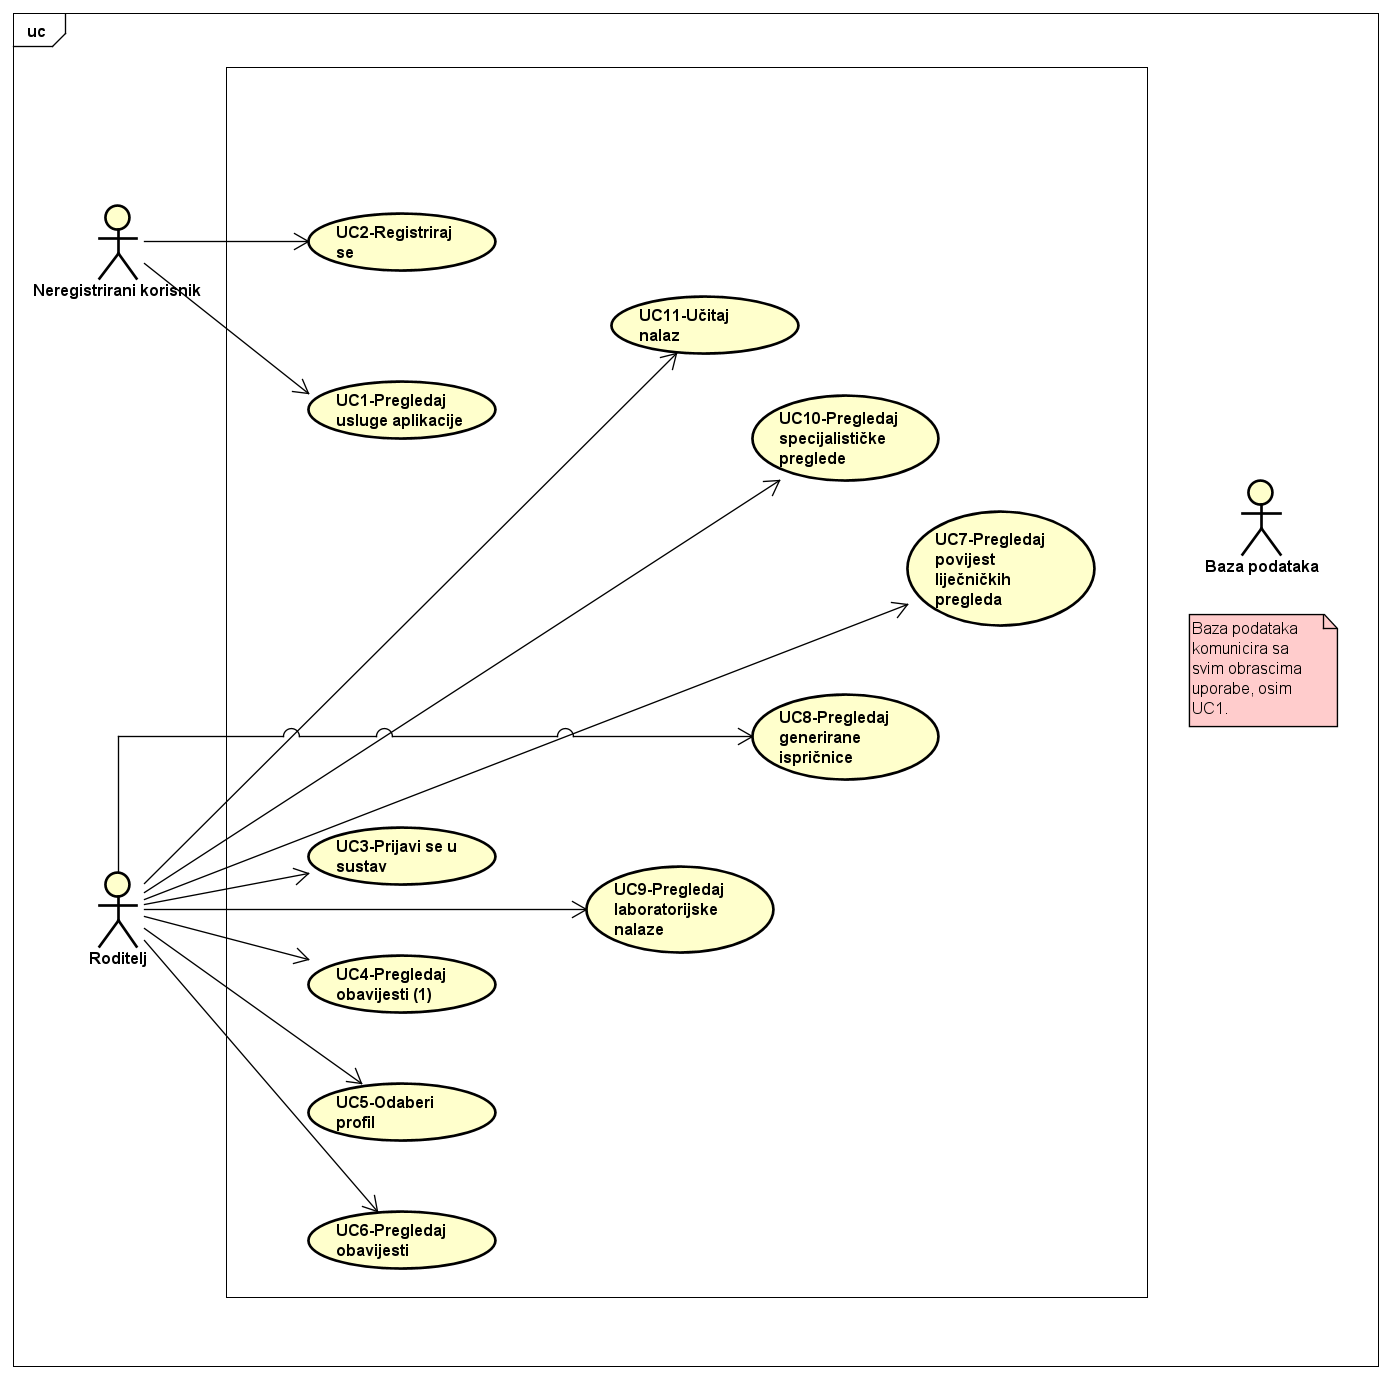
\includegraphics[scale=0.4]{dijagrami/usecase1.PNG} %veličina slike u odnosu na originalnu datoteku i pozicija slike
						\centering
						\caption{Dijagram obrazaca uporabe, funkcionalnost nereg. korisnika i Roditelja}
						\label{fig:useacase1}
					\end{figure}
					
					%unos slike
					\begin{figure}[H]
						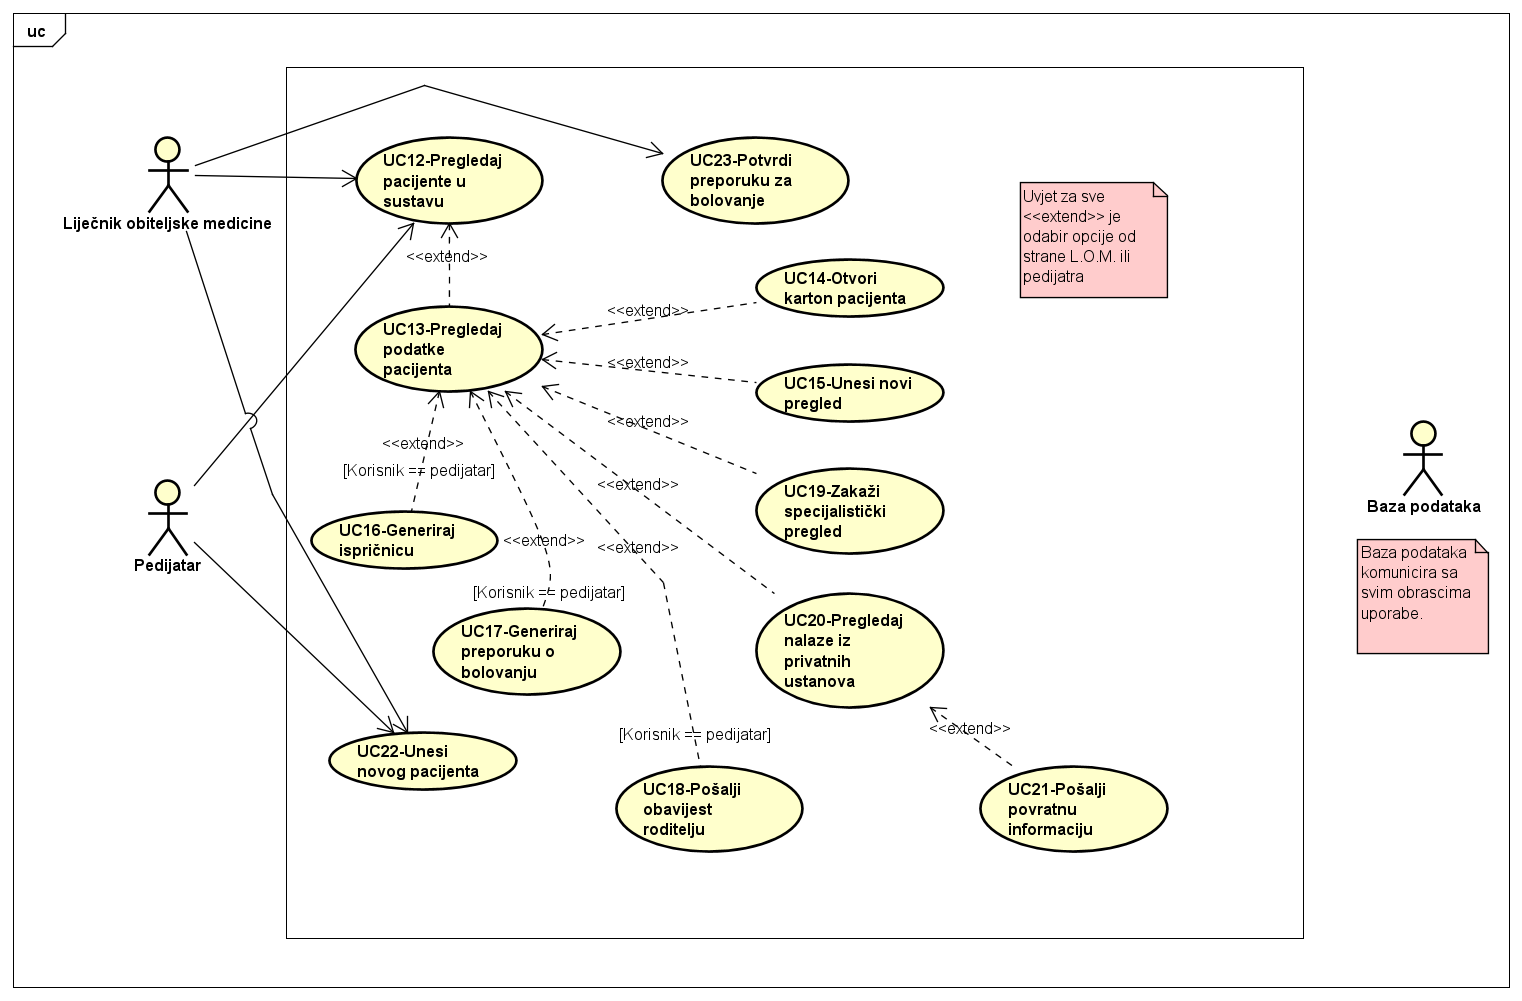
\includegraphics[scale=0.4]{dijagrami/usecase2.PNG} %veličina slike u odnosu na originalnu datoteku i pozicija slike
						\centering
						\caption{Dijagram obrazaca uporabe, funkcionalnost Pedijatra i L.O.M.}
						\label{fig:usecase2}
					\end{figure}
					
					%unos slike
					\begin{figure}[H]
						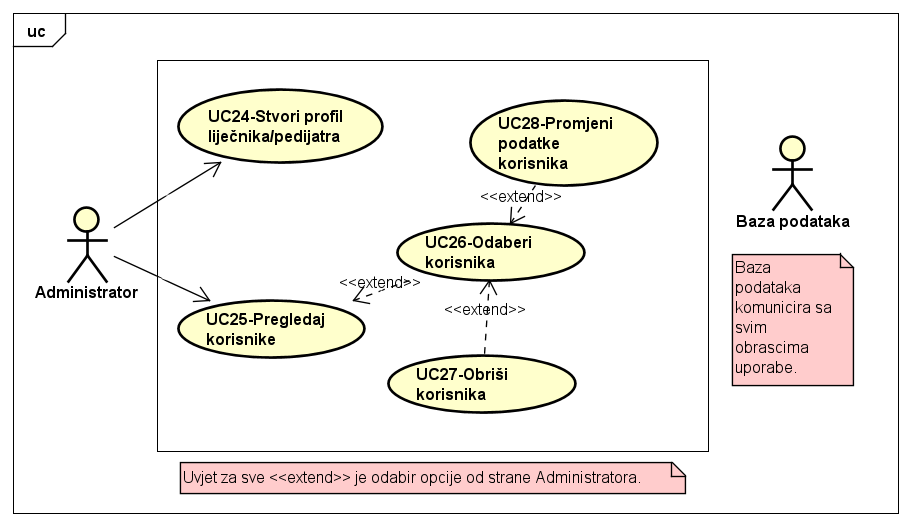
\includegraphics[scale=0.5]{dijagrami/usecase3.PNG} %veličina slike u odnosu na originalnu datoteku i pozicija slike
						\centering
						\caption{Dijagram obrazaca uporabe, funkcionalnost Administratora}
						\label{fig:usecase3}
					\end{figure}
				\eject		
				
			\subsection{Sekvencijski dijagrami}
				\textbf{Sekvencijski dijagram - Obrasci uporabe UC3, UC4, UC5, UC6, UC7 (Od prijave do prikaza povijesti liječničkih pregleda)}\newline
					\text Roditelj prvo šalje zahtjev za prijavom, nakon čega ga sustav prebacuje na ekran za prijavu. Roditelj unosi podatke, koje sustav uzima i provjerava u bazi. Ako su ispravni, sustav dobavlja popis profila vezanih uz korisnički račun i popis svih obavijesti vezanih uz račun roditelja, nakon čega sustav otvara prikaz profila i obavijesti. Kada roditelj odabere jedan od računa, dobavljaju se podaci o tom računu, te popis obavijesti vezanih samo uz taj račun, i zatim se roditelju otvara profil, s prikazanim obavijestima. Roditelj odabire opciju za prikaz povijesti liječničkih pregleda. Sustav nakon toga dobavlja medicinski karton tog profila, nakon čega pomoću identifikatora kartona dobavlja popis obavljenih pregleda. Korisniku se otvara prikaz povijest liječničkih pregleda. \\
					
					%unos slike
					\begin{figure}[H]
						\includegraphics[scale=0.4]{dijagrami/rodseq1.PNG} %veličina slike u odnosu na originalnu datoteku i pozicija slike
						\centering
						\caption{Sekvencijski dijagram prikaza pregleda}
						\label{fig:seq1}
					\end{figure}
					\clearpage
				\textbf{Sekvencijski dijagram - Obrasci uporabe UC13, UC15, UC16 (Odabir pacijenta, novi pregled i ispričnica)}\newline
				\text Na popisu pacijenata pedijatar odabire jednog. Sustav pristupa bazi podataka iz koje vraća podatke o pacijentu, koji se zatim koriste pri stvaranju prikaza osobnih podataka pacijenta. Ako na profilu pacijenta pedijatar odabere opciju za unos novog pregleda, sustav dobavlja podatke o pacijentu ponovno iz baze, te ih zapisuje u polja za podatke pacijenta u prikazu koji stvara za pedijatra. U taj prikaz pedijatar, u za to određena polja, unosi podatke o pregledu. Ti podaci, kao i podaci pacijenta, koriste se u stvaranju novog objekta pregleda koji se sprema u bazu podataka. Pedijatra se nakon potvrde uspješnog spremanja u bazu vraća na profil pacijenta. [Bitno! UC13 i UC15 na identičan način funkcioniraju i za L.O.M.] Ako pedijatar odabere opciju za generiranje ispričnice, sustav iz baze prenosi podatak o kontaktu škole, koji se zapisuje u polje u prikazu za stvaranje nove ispričnice. U tom prikazu pedijatar ispunjava ostala polja, primarno opis razloga izdavanja ispričnice. Ispričnica se generira, prilikom čega se prvo šalje školi, a zatim sprema u bazu. Nakon primljene potvrde o uspješnom spremanju u bazu, sustav vraća pedijatra na profil pacijenta.
				
				%unos slike
				\begin{figure}[H]
					\includegraphics[scale=0.35]{dijagrami/pedseq1.PNG} %veličina slike u odnosu na originalnu datoteku i pozicija slike
					\centering
					\caption{Sekvencijski dijagram osnovnih funkcionalnosti pedijatra}
					\label{fig:seq2}
				\end{figure}
				\clearpage
				
				\textbf{Sekvencijski dijagram - Obrasci uporabe UC17 i UC23 (Generiranje i potvrda preporuke o bolovanju)}\newline
					\text Na profilu pacijenta pedijatar odabire opciju generiraj preporuku za bolovanje. Sustav iz baze podataka dohvaća podatke o roditelju pacijenta. Iz njih se čuvaju email adresa poslodavca i identifikator liječnika. Pedijatru se otvara prikaz u kojem ispunjava podatke o preporuci o bolovanju (npr. razlog i trajanje, te ime i prezime roditelja). Nakon potvrde generiranja preporuke, ona se sprema u bazu podataka.
					Kada liječnik želi pristupiti preporukama o bolovanju, on odabire opciju na svom izborniku. Kada odabere tu opciju, iz baze se dohvaćaju sve preporuke o bolovanju koje su povezane na doktora putem njegovog identifikatora. Za svaku doktor može odabrati opciju "Potvrdi" ili "Odbij". Prilikom potvrde se generira i šalje doznaka o bolovanju poslodavcu, nakon čega se preporuka briše iz baze. U slučaju odbijanja, preporuka se isto briše iz baze, bez slanja.
					%unos slike
					\begin{figure}[H]
						\includegraphics[scale=0.4]{dijagrami/pedseq2.PNG} %veličina slike u odnosu na originalnu datoteku i pozicija slike
						\centering
						\caption{Sekvencijski dijagram stvaranja i potvrde preporuke o bolovanju}
						\label{fig:seq3}
					\end{figure}
					\clearpage
					
				\textbf{Sekvencijski dijagram - Obrasci uporabe UC11, UC20 i UC21 (\textit{Upload} nalaza, pregled svih nalaza i opcionalno slanje povratne informacije)}\newline
					\text Roditelj može na meniju otvorenog profila odabrati opciju za učitavanje nalaza od privatnika. Sustav roditelju otvara prikaz za \textit{upload} s poljima za dodatne informacije. Nakon što roditelj odabire opciju "Učitaj", stvara se novi objekt privatnog nalaza, koji se povezuje na medicinski karton pacijenta, čiji je identifikator jedno od polja u objektu Roditelj/Dijete. Pedijatar/liječnik može na otvorenom profilu pacijenta odabrati opciju za prikaz nalaza od privatnika. U tom slučaju sustav iz baze podataka dobavlja popis, i prikazuje ga pedijatru/liječniku, nakon čega pedijatar/liječnik može otvoriti svaki pojedinačno. Nakon otvaranja detaljnog prikaza nalaza, pedijatar može odabrati opciju za slanje povratne informacije. Nakon toga mu sustav otvara prikaz za slanje obavijesti. Nakon ispunjavanja podataka obavijesti i pritiska opcije za slanje, sustav dobavlja OIB koji je potreban za stvaranje objekta obavijesti iz baze, nakon čega sprema obavijest. [Važno: postupak čitanja obavijesti već je opisan u sekvencijskom dijagramu (Slika 3.4)]
					%unos slike
					\begin{figure}[H]
						\includegraphics[scale=0.4]{dijagrami/pedseq3.PNG} %veličina slike u odnosu na originalnu datoteku i pozicija slike
						\centering
						\caption{Sekvencijski dijagram rada s privatnim nalazima}
						\label{fig:seq4}
					\end{figure}
					\clearpage
				
					
				\eject
	
		\section{Ostali zahtjevi}
			 
			 \text Aplikacija treba biti prilagođena radu na različitim uređajima, specifično na računalima, tabletima i mobitelima. \\
			 \text Aplikacija treba podržavati više korisnika u isto vrijeme. Maksimalan broj podržanih korisnika nije definiran. \\
			 \text Aplikacija treba biti izvedena kao web aplikacija. Siguran pristup mora biti osiguran korisničkim imenom i lozinkom, no nisu definirani zahtjevi dodatne zaštite.
			 
			 
			 
	